\section{Product Perspective}
\label{sec:product_Perspective}

\subsection{Scenarios}
\label{subsec:scenarios}

\item \textbf{1st Scenario: User Registration and Profile Management}\\
Elena Rossi, an avid cyclist and member of a local biking association, decides to join the BBP platform to keep track of her cycling activity and share information with other bikers. 
Upon opening the application, she selects the \textit{Sign Up} option. BBP prompts her to enter her personal details such as name, email, and password. Once the verification process is complete, Elena accesses her personal profile page. She updates her information, adds a short description of her cycling interests, and enables location permissions. From this moment, Elena becomes a registered user, able to record her trips and contribute data about bike paths.

\item \textbf{2nd Scenario: Recording and Viewing a Trip with Statistics}\\
Fausto Coppi is training for his next Tour. Fausto decides to record his rides using BBP. Before starting, he opens the app and presses \textit{Start Trip Recording}. 
During the ride, the app collects GPS data to track his route and speed. Once he arrives at his destination, he presses \textit{Stop}. The system automatically saves his trip and calculates key statistics: total distance, average speed, and travel time. Fausto later accesses his trip history, where he can review all his recorded rides, compare performances, and track his progress over time.

\item \textbf{3rd Scenario: Manual Insertion of Path Information}\\
During one of her rides, Federica Conti, an environmental engineering student and urban cyclist, discovers a newly built cycling lane that is not yet available on BBP’s map. 
After returning home, she opens the \textit{Add Path} section and manually inserts the details: the street names, total distance, surface quality, and current condition (e.g., \textit{Optimal}). She also reports a minor obstacle—a small pothole near a crossroad. After submitting, the system stores the path information, marking it as pending publication until Federica decides to make it public.

\item \textbf{4th Scenario: Automatic Path Detection and User Confirmation}\\
Marco Bianchi, a competitive cyclist who trains daily, prefers to let the system work automatically. 
Before starting his ride, he opens BBP and enables the \textit{Automatic Path Tracking} option, which allows the app to record his route and detect potential obstacles without manual intervention. 
When he starts cycling, BBP detects his movement and recognizes that he is riding. The system begins to collect GPS data and sensor readings from the accelerometer and gyroscope. 
After completing the trip, Marco receives an automatic summary of the detected path and potential obstacles identified by the sensors. He notices that BBP has mistakenly flagged a bump as a pothole, so he corrects the information before confirming the path. Once validated, the path is saved in his account..

\item \textbf{5th Scenario: Publishing a Recently Completed Path}\\
After reviewing and confirming the data from her latest ride, Sofia Moretti, an experienced city biker, decides to share it immediately with other cyclists. 
As soon as she finishes the trip and validates the automatically collected information, BBP prompts her with an option to \textit{Publish Path Information}. 
Sofia confirms the publication request, and the system instantly adds the path data to the public database, updating the collaborative map of available routes. 
Within moments, the new path becomes visible to all users of the platform.

\item \textbf{6th Scenario: Publishing a Previously Stored Path}\\
Two weeks later, Andrea Ricci, a cycling enthusiast who often explores rural routes, revisits one of his older recorded trips, which he never published. He reviews the path, adds updated comments about its current condition, and decides to share it with the community. 
He clicks \textit{Publish}, and BBP processes the data, making it available in the shared inventory. The system automatically merges his contribution with existing information about the same route, if available, ensuring that the most recent and confirmed data are displayed.

\item \textbf{7th Scenario: Consulting and Choosing a Path (Registered User)}\\
Francesco Leone, a registered cyclist who commutes daily by bike, plans a weekend trip across the city. He logs into BBP and specifies his origin and destination. 
The system searches the database for suitable routes and displays multiple options on the map, sorted by their score—considering factors such as safety, condition, and efficiency. 
Since Francesco’s profile indicates a preference for smoother surfaces and minimal traffic, BBP’s recommendation system automatically prioritizes such routes in the results. 
After reviewing the suggested paths, Francesco selects one and saves it as his chosen itinerary for the day.

\item \textbf{8th Scenario: Consulting and Choosing a Path (Unregistered User)}\\
Marta Villa, a casual cyclist who enjoys leisure rides on weekends, wants to discover new paths without creating an account. She opens the BBP app without logging in and accesses the public map. 
BBP displays all available paths but without personalized recommendations. Marta browses the map, filters by \textit{Optimal} status, and selects a route along the lakeside. Although she cannot record trips or add data, she can still view general information, such as total length, average condition, and user comments.

\item \textbf{9th Scenario: Updating Information on an Existing Path}\\
During a weekly commute, Tommaso Greco, a frequent user of BBP, rides along a route previously marked as \textit{Optimal}. He notices that a section of the track has recently deteriorated and requires maintenance. 
Once he finishes the ride, he opens BBP and selects \textit{Update Path Information}. He searches for the existing path and updates its condition from \textit{Optimal} to \textit{Requires Maintenance}. 
The system records his update and automatically aggregates it with reports from other users who have recently traveled the same route. 
By considering both the number of confirmations and the recency of the available data, BBP determines the most reliable current status of the path and updates its classification accordingly.

\end{itemize}

\subsection{Domain-level Class Diagram}
\label{subsec:domain_level_class_diagrams}

\begin{figure}[H]
    \begin{center}
        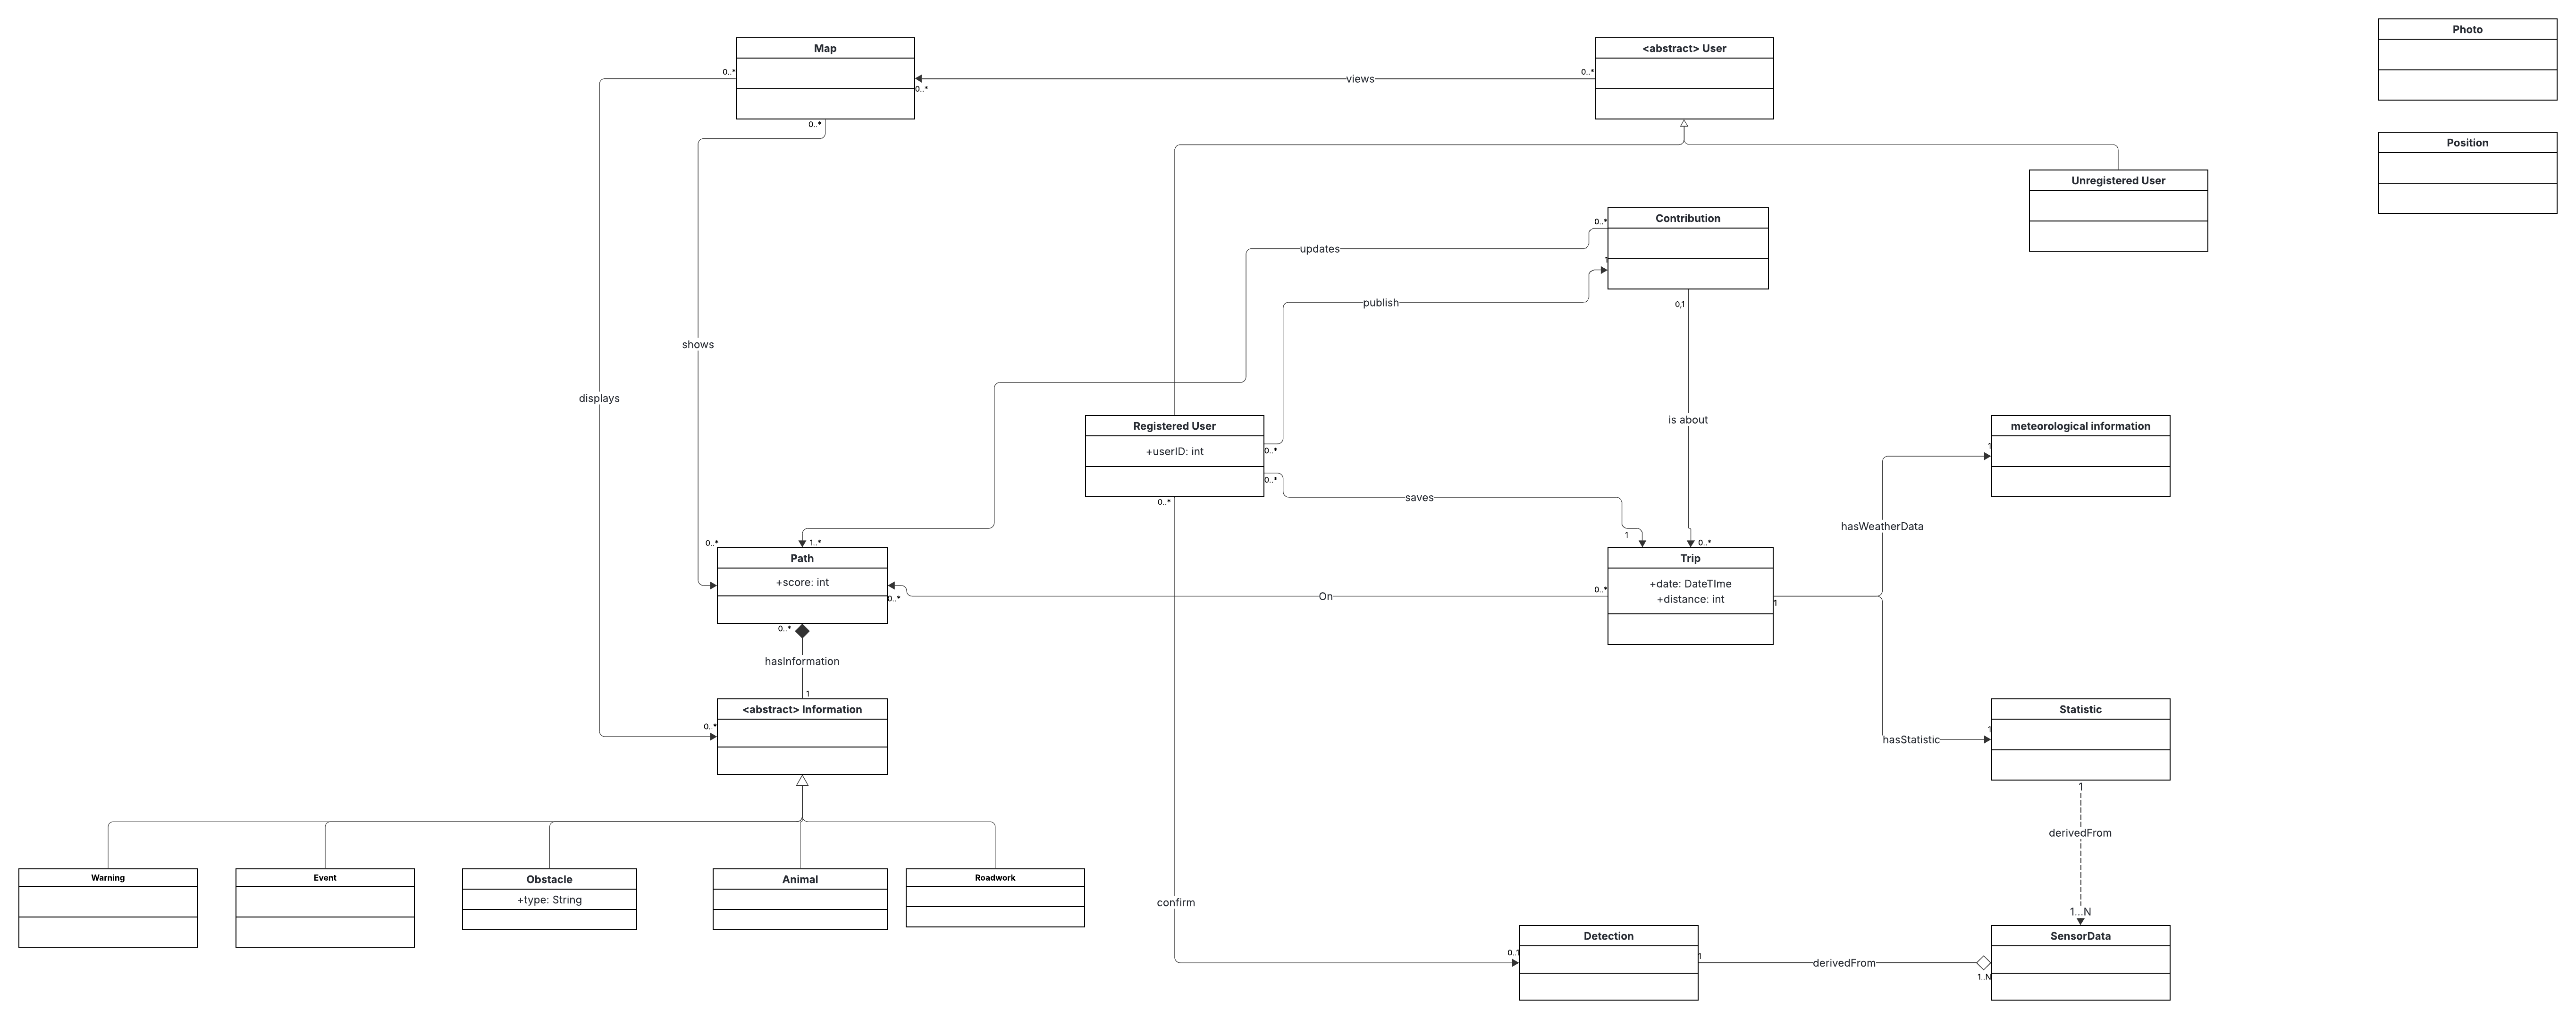
\includegraphics[width=0.9\linewidth]{RASD/Version1.0/images/UML class.png}
        \caption{Domain-Level Class Diagram.}
        \label{fig:domain_level_class_diagrams}
    \end{center}
\end{figure}

The entities interacting with the system are modeled through a hierarchical user structure in order to capture the capabilities and permissions required by the application. At the top level, the abstract User class generalizes any individual who accesses the application, whether simply browsing the map and available paths or actively contributing new information. In particular, the \textit{RegisteredUser} class extends User and enables all advanced features such as recording trips, confirming detections, and publishing contributions, while \textit{UnregisteredUser} supports basic navigation and map viewing functions.


The central concept of the application is the \textit{Contribution}, representing any information about the cycling network produced by a user or inferred automatically from sensor data. A contribution is always associated with a Path, and describes events or obstacles that affect that route. Contributions can be published directly by registered users (manual contributions), or generated via the confirmation of automatic detections performed during a trip. Each contribution updates the set of facts associated with a path and can include attachments such as photos or geographical positions for increased detail. The publication mechanism allows users to decide when their contributions become visible to all map viewers and impact the quality and usability scoring of each path segment.


The \textit{Path} entity models the infrastructure of the cycling network, comprising static segments that connect origins and destinations. Each path aggregates multiple pieces of Information—an abstract class that generalizes the different kinds of facts and events reported about the network. Its concrete subclasses include \textit{Warning, Event, Obstacle, Animal, and Roadwork}, each expressing specific types of phenomena detected or reported. The composition between path and information structures a dynamic collective history, while an explicit score attribute summarizes overall path safety or comfort, based on contributions and validations received.


The \textit{Trip} entity represents a specific cycling session recorded by a registered user. Each trip is associated with the user who performed it, stores basic data such as the date and distance, and can be complemented by additional statistical summaries (via the Statistic class) and meteorological data. Statistics are derived from raw \textit{SensorData} sampled during the ride, allowing the application to analyze detailed route conditions, travel patterns, and support more accurate detections of issues.


The detection process is modeled by the \textit{Detection} class, which represents the outcome of automatic analysis on a user's trip. When sensor data collected during a trip suggests the presence of a possible obstacle, the system generates a detection linked to that trip and to the affected path segment. Detections remain private and require explicit user confirmation: when a registered user reviews their trip, they confirm whether the suggested detection was a genuine obstacle encountered during the ride. Only upon confirmation does the system create or update a related Contribution, associating the appropriate \textit{Information} subtype (such as \textit{Obstacle} or \textit{Roadwork}) to the Path. Unconfirmed or rejected detections do not affect public contributions and path information. In this way, detections act as an intermediate, trip-specific representation that requires user validation, while contributions are the authoritative model for updating the infrastructure database.


The \textit{Map} entity models the application’s visualization layer. It displays all available paths, their associated contributions and information, and overlays real-time obstacles and statistics to let users plan their journeys. Any user can select a start and end point on the map; the system calculates the path, presents the obstacles detected, and helps choose the safest or most comfortable route.


Optional multimedia and localization enrichment is supported by the \textit{Photo} and \textit{Position} entities. Positions specify geographic coordinates for a point along a path, while photos can visually document the situation encountered. By associating these elements with contributions or information items, the system ensures precise localization and improves the transparency and reliability of the data shared across the platform.

